\documentclass[twoside]{article}
\input{ISC18-english.sty}
%%%%%%%%%%%%%%%%%%%%%%%%%%%%  Make sure to compile twice for proper cross-references. %%%%%%%%%%%%%%%%%%%%%%%
%%%%%%% For proper display of references, compile the document twice. %%%%%%%%%%%%%%%%%%%%%
%%%%%%%%%%%%%%% If using TeX Live, compile using pdflatex command %%%%%%%%%%%%%%%%%%%%%%%
\begin{document}
\thispagestyle{empty}
%%%%%%%%%%%%%%%%% Article title header  %%%%%%%%%%%%%%%%%%%%
\fancyhead[LE]{High-Resolution Spectral Estimation}
%%%%%%%%%%%%%%%%% Article authors header   %%%%%%%%%%%%%%%%%%%%
\fancyhead[RO]{A. R. Nematollahi}
\begin{center}
{
\includegraphics [height=25mm, width=150.3mm] {Images/isc18E}} \\
\vspace*{-1.8cm}
%\begin{center}
%\color{blue}
%{\hspace{0.1cm}\rule{\textwidth}{1mm}}\\
%\end{center}
\vspace*{4cm}
%%%%%%%%%%%%%%%%% Article title  %%%%%%%%%%%%%%%%%%%%
{\Large \bf High-Resolution Spectral Estimation of Univariate and Multivariate Stationary Time Series}\\
%%%%%%%%%%%%%%%%% Article authors and affiliations %%%%%%%%%%%%%%%%%%%%
%{\bf
%A. R. Nematollahi \footnote[1]{{\bf Corresponding Author:} {\tt ar.nematollahi@shirazu.ac.ir }} \\
%Departement of Statistics, Shiraz University, \\ Shiraz, Iran.}
\end{center}
\rule{\textwidth}{0.2mm}\\
%%%%%%%%%%%%%%%%% Article abstract  %%%%%%%%%%%%%%%%%%%%
\noindent{\bf Abstract:}\\
This study evaluates spectral density estimation techniques for stationary time series, with an emphasis on high-resolution methods. Classical approaches often have difficulty resolving closely-spaced frequency components when data is limited. Through controlled simulations, we compare these traditional techniques against high-resolution estimators and show that the latter consistently deliver clearer, more distinct frequency estimates. The methods are also extended to multivariate time series, demonstrating their practical value in complex signal characterization.



\noindent{\bf Keywords:}
Stationary time series, Spectral density, Capon's estimate, High resolution estimate, Block-Toeplitz matrix, Periodogram. \\
\noindent{\bf Mathematics Subject Classification (2010):} $\rm 62M15$, $\rm 62G07$, $\rm 15B05$. \\
\hspace{1cm}\rule{\textwidth}{0.2mm}\\
%%%%%%%%%%%%%%
\section{Introduction}



Time series analysis is carried out in two main domains: the time domain, based on correlation, and the frequency domain, based on spectral analysis. Although engineers and statisticians may use different terminology, both views are essential for understanding complex systems. Spectral analysis aims to determine how signal power is distributed across frequency, a problem known as spectral density estimation, which involves recovering this distribution from finite measured data.



Spectral analysis is widely used across many fields. In economics and meteorology, it uncovers hidden periodicities. In radar, sonar, and seismology, it helps with target localization and movement analysis. In medicine (e.g., ECG and EEG) and control systems, it aids in diagnosing system behavior. For comprehensive reviews, see \cite{Kay:1988}, \cite{Marple:1987}, \cite{StoicaMoses:1997}, \cite{StoicaMoses:2005}, \cite{PercivalWalden:1993}, \cite{Carbone:2022}, and \cite{ShumwayStoffer:2025}.



Spectral estimation methods fall into two broad categories: parametric and nonparametric. Parametric approaches, such as AR and Maximum Entropy methods, fit models to the data and depend on correct model selection. Nonparametric methods, like windowed periodograms, estimate the spectrum directly without assuming a specific model. While both are foundational, they often have difficulty resolving closely-spaced frequency components due to resolution limits, especially with short data records.



This paper focuses on High-Resolution spectral estimation techniques, which offer a robust alternative for identifying narrow spectral peaks. We evaluate these methods against traditional approaches through a series of comparative simulation studies. Finally, we extend this analysis to the context of multivariate time series, demonstrating the practical utility of High-Resolution techniques in complex signal characterization.



\section{Preliminaries}
Let $\{X_t\}_{t \in \mathbb{Z}}$ be a real-valued, zero-mean, discrete-time stationary process with finite variance, $E\vert{}X_t\vert{}^2 < \infty$,  where $\mathbb{Z}$ stands for all integers. Given an autocovariance function $R(\tau) = E(X_t X_{t+\tau})$ that satisfies $\sum_{\tau=-\infty}^{\infty} \vert{}R(\tau)\vert{} < \infty$, the power spectral density (PSD) function is defined as:
\begin{equation}
h(\omega) = \frac{1}{2\pi} \sum_{\tau=-\infty}^{\infty} R(\tau) e^{-i\omega \tau}, \quad \omega \in (-\infty, \infty).
\end{equation}



Here, $\omega$ denotes the angular frequency (with cyclic frequency $f = \omega/2\pi$ and period $T = 1/f$). Absolute summability of $R(\tau)$ ensures uniform convergence, making $h(\omega)$ bounded and continuous. Due to stationarity, $h(\omega)$ is non-negative, even, and $2\pi$-periodic, so it is fully described over $\omega \in [0, \pi]$. The autocovariance is recovered via the inverse Fourier transform:
\begin{equation}
R(\tau) = \int_{-\pi}^{\pi} h(\omega) e^{i\omega \tau} \,d\omega, \qquad \tau \in \mathbb{Z}.
\end{equation}



At $\tau = 0$, this gives the variance: $R(0) = \text{var}(X_t) = \int_{-\pi}^{\pi} h(\omega) \, d\omega$. The term "power" originates from engineering, where $h(\omega)$ describes how variance is distributed across frequencies. A peak in the spectrum indicates a strong contribution to variance at that frequency. While the autocovariance and spectrum are theoretically equivalent, they offer complementary views: the time domain is better for temporal analysis, and the frequency domain excels at revealing hidden periodicities.



\section{Parametric Methods}
Parametric spectral estimation techniques are based on the assumption that the underlying stationary time series is generated by a model with a known functional form. The estimation procedure involves two primary steps: identifying the model parameters and subsequently deriving the spectral density from the fitted model. Unlike nonparametric approaches, which estimate the spectrum directly from the data without prior structural assumptions, parametric methods rely on the adequacy of the assumed model. When the model accurately represents the underlying physical process, parametric techniques can provide spectral estimates with superior statistical precision and resolution.



Typically, this process involves fitting an Autoregressive Moving Average (ARMA) model to the observed data. The model order is systematically selected using information criteria, such as the bias-corrected Akaike Information Criterion (AICC) (\cite{Akaike:1973}).
For an $p$th-order autoregressive [AR$(p)$] model, the spectral density estimator $\widehat{h}_p(\omega)$ is defined as:
\begin{equation}
\widehat{h}_p(\omega) = \frac{\widehat{v}_p}{2\pi} \cdot \left| 1 - \sum_{k=1}^{p} \widehat{\phi}_{pk} e^{-ik\omega} \right|^{-2},
\end{equation}
where $\widehat{\boldsymbol{\phi}}_p = (\widehat{\phi}_{p1}, \dots, \widehat{\phi}_{pp})^{\mathsf{T}}$ is the vector of estimated AR coefficients, and $\widehat{v}_p$ denotes the estimated innovation variance. This estimator is mathematically equivalent to the Maximum Entropy Method (MEM), which maximizes the spectral entropy subject to given autocovariance constraints (see \cite{BrockwellDavis:1991}).



While the Yule-Walker approach provides one path to estimating the coefficients $\widehat{\boldsymbol{\phi}}_p$, the Burg method is frequently preferred in spectral analysis. Unlike Yule-Walker, which implicitly relies on windowing the autocovariance estimates and may lead to spectral line splitting or bias in short records, the Burg method estimates the AR parameters by minimizing the sum of the forward and backward prediction error powers. This approach ensures high-resolution spectral peaks and maintains the stability of the resulting AR model, effectively resolving closely spaced frequency components that traditional estimators might merge, see \cite{BrockwellDavis:1991}.



When the process exhibits complex spectral features, such as sharp peaks and deep nulls, AR models may be insufficient. In such cases, the more flexible ARMA$(p,q)$ model is preferred. The Maximum Likelihood ARMA (MLARMA) spectral estimate is given by:
\begin{equation}
\widehat{h}_{p,q}(\omega) = \frac{\widehat{\sigma}^2}{2\pi} \cdot \frac{\left| 1 + \sum_{k=1}^{q}\widehat{\theta}_{qk} e^{-ik\omega} \right|^2}{\left| 1 - \sum_{k=1}^{p} \widehat{\phi}_{pk} e^{-ik\omega} \right|^2},
\end{equation}
where $\widehat{\boldsymbol{\phi}}_p = (\widehat{\phi}_{p1}, \dots, \widehat{\phi}_{pp})^{\mathsf{T}}$ and $\widehat{\boldsymbol{\theta}}_q = (\widehat{\theta}_{q1}, \dots, \widehat{\theta}_{qq})^{\mathsf{T}}$ are the estimated AR and MA coefficient vectors, respectively, and $\widehat{\sigma}^2$ is the estimated innovation variance of the ARMA process, with parameters obtained via maximum likelihood estimation. Although MLARMA is highly flexible, it is computationally intensive. As a computationally efficient alternative, Moving Average (MA) estimators or indirect numerical methods (see \cite{Stoicaetal:2000} and \cite{Dumitrescuetal:2001}) are often employed when the MA($\infty$) representation of the process exhibits rapidly decaying coefficients. These methods provide a balance between statistical accuracy and computational efficiency, particularly for large datasets.



\section{Nonparametric Methods}
Nonparametric spectral estimation aims to estimate the power spectral density (PSD) without assuming a specific data-generating model. The fundamental tool in this approach is the periodogram, $I_n(\omega)$, defined for a data sequence $\{X_1, \ldots, X_n\}$ as:
\begin{equation}
I_n(\omega) = \frac{1}{n} \left| \sum_{t=1}^n X_t e^{-it\omega} \right|^2 = \sum_{\tau = -(n-1)}^{n-1} \widehat{R}(\tau) e^{-i\tau \omega},
\end{equation}
where $\widehat{R}(\tau)$ is the sample autocovariance function. While $I_n(\omega)$ is an asymptotically unbiased estimator of $2\pi h(\omega)$, it lacks consistency, its variance does not vanish as $n \to \infty$, causing the spectral estimate to fluctuate wildly. Consequently, modification via smoothing is necessary. Smoothing can be performed either in the time domain (using lag windows) or the frequency domain (spectral averaging).



\subsection{Lag Window Estimators}



To reduce variance, we apply a weight function $\lambda(\tau)$ to the autocovariances, effectively truncating the series at a lag $M < n$:
\begin{equation}
\widehat{h}(\omega) = \frac{1}{2\pi} \sum_{\tau=-M}^{M} \lambda(\tau) \widehat{R}(\tau) e^{-i\tau \omega}.
\end{equation}



Commonly used lag windows $\lambda(\tau)$ include:



\begin{itemize}
    \item \textbf{Truncated (Rectangular):} $\lambda(\tau) = 1 \quad \text{for } |\tau| \le M$, and $0$ otherwise.
    \item \textbf{Triangular (Bartlett):} $\lambda(\tau) = 1 - \frac{|\tau|}{M} \quad \text{for } |\tau| \le M$.
    \item \textbf{Hamming:} $\lambda(\tau) = 0.54 + 0.46\cos\left(\frac{\pi \tau}{M}\right) \quad \text{for } |\tau| \le M$.
    \item \textbf{Hanning:} $\lambda(\tau) = 0.5 + 0.5\cos\left(\frac{\pi \tau}{M}\right) \quad \text{for } |\tau| \le M$.
    \item \textbf{Blackman-Tukey:} $\lambda(\tau) = 0.42 + 0.5\cos\left(\frac{\pi \tau}{M}\right) + 0.08\cos\left(\frac{2\pi \tau}{M}\right) \quad \text{for } |\tau| \le M$.
    \item \textbf{Parzen:} A piecewise polynomial function emphasizing central lags.
    \item \textbf{Bartlett-Priestley:} An optimal window derived by minimizing the relative mean square error (see \cite{Priestley:1962}).
\end{itemize}



The choice of bandwidth $M$ involves a fundamental trade-off: a smaller $M$ reduces variance but increases bias (oversmoothing), whereas a larger $M$ preserves spectral features but increases variance (erratic behavior). A common heuristic is $M \approx 2\sqrt{n}$.



\subsection{Spectral Average Estimators (Daniell Window)}



Alternatively, one can achieve consistency by smoothing the periodogram in the frequency domain:
\begin{equation}
\tilde{h}(\omega_j) = \frac{1}{2\pi} \sum_{|k| \le M} W_n(k) I_n(\omega_{j+k}),
\end{equation}
where $\{W_n(k)\}$ are non-negative weights satisfying:
\begin{itemize}
    \item $W_n(k) = W_n(-k)$,
    \item $\sum_{|k| \le M} W_n(k) = 1$,
    \item $\sum_{|k| \le M} W_n^2(k) \to 0$ as $n \to \infty$.
\end{itemize}



This approach effectively averages neighboring periodogram ordinates, which are approximately independent, to construct a stable and consistent estimate of the PSD.





\subsection{High-Resolution Spectral Estimation}
Classical spectral estimation methods often fail to resolve closely-spaced spectral peaks, particularly when the sample size $n$ is small. High-resolution methods overcome these limitations by moving beyond the periodogram's inherent resolution constraints. Two prominent approaches in this category are the Capon (Minimum Variance) estimator and the Pisarenko estimator.



\textbf{1. The Capon (Minimum Variance) Estimator}



Proposed by \cite{Capon:1969}, this method, often termed the Minimum Variance Distortion less Response (MVDR) estimator, estimates the spectrum by minimizing the output power of a linear filter under the constraint that the signal at the frequency of interest passes with unity gain.Let $\{X_t\}$ be a process with autocovariance matrix $\mathbf{R}_p$. For an $AR(p)$ model, the linear filter output is $\hat{X}_n = \mathbf{a}_p^{\mathsf{T}} \mathbf{X}_n$, where $\mathbf{X}_n = (X_{n-1}, \dots, X_{n-p})^{\mathsf{T}}$ and $\mathbf{a}_p$ is the coefficient vector. Minimizing the variance $E\vert{}\hat{X}_n\vert{}^2 = \mathbf{a}_p^{\mathsf{T}} \mathbf{R}_p \mathbf{a}_p$ subject to $\mathbf{a}_p^{\mathsf{T}} \mathbf{L}_p(\omega) = 1$, where $\mathbf{L}_p(\omega) = (1, e^{i\omega}, \dots, e^{ip\omega})^{\mathsf{T}}$ is the direction vector, yields the optimal weight vector:
\begin{equation}
\mathbf{a}_{MV} = \frac{\mathbf{R}_p^{-1} \mathbf{L}_p(\omega)}{\mathbf{L}_p^{\mathsf{T}}(\omega) \mathbf{R}_p^{-1} \mathbf{L}_p(\omega)}.
\end{equation}



Substituting this into the variance expression gives the Capon spectral density estimate:
\begin{equation}
h_{\mathrm{Cap}}(\omega) = \frac{1}{\mathbf{L}_p^{\mathsf{T}}(\omega) \mathbf{R}_p^{-1} \mathbf{L}_p(\omega)}
= \left( \mathbf{L}_p^{\mathsf{T}}(\omega) \mathbf{R}_p^{-1} \mathbf{L}_p(\omega) \right)^{-1}.
\label{eq:capon}
\end{equation}
Note that while the Capon estimator is typically applied to a local window of length $p$ (where $p < n$), the eigenvalue-based approach discussed below allows for a broader analysis using the full sample size $n$.



\textbf{Note}: In telecommunications, this is closely related to the MUSIC algorithm, which utilizes the eigen decomposition of $\mathbf{R}_p$ to provide even higher resolution.



\textbf{2. The Pisarenko and General Estimators}



\cite{Pisarenko:1972}  provided a distinct perspective by relating spectral estimation to the eigenvalues of the Toeplitz autocovariance matrix $\mathbf{R}_n$, defined by the elements $R(t-s)$. A foundational framework for this approach was established by \cite{SubbaRaoGabr:1989}, who bridged the gap between engineering-based high-resolution techniques and statistical time series analysis. They demonstrated that spectral estimators can be interpreted through the eigenvalues $\{\lambda_{n,j}\}$ of $\mathbf{R}_n$. Using the asymptotic equivalence between Toeplitz matrices and circular symmetric matrices (Gray, 1972), they expressed the "truncated spectral density function" as:
\begin{equation}h_n(\omega_l) = \frac{1}{4\pi} \left( \lambda_{n,0} A_{n,0}(\omega_l) + \sum_{j=1}^{(n-1)/2} (\lambda_{n,2j} + \lambda_{n,2j-1}) A_{n,2j}(\omega_l) \right),
\end{equation}
where $A_{n,j}(\omega_l)$ represents a weighting function derived from the Fejér kernel, $F_n(\theta) = \frac{1}{2\pi n} \frac{\sin^2(n\theta/2)}{\sin^2(\theta/2)}$. Since $h_n(\omega_l)$ is a linear combination of the eigenvalues $\lambda_{n,j}$, this suggests that replacing these eigenvalues with a non-linear function $G(\cdot)$ can yield a broader class of estimators. Specifically, for a strictly monotone continuous function $G(\cdot)$ and its inverse $g(\cdot)$, the general form of the Pisarenko-type estimator is defined as:
\begin{equation}h_{n,\mathrm{P}}(\omega_l) = g\left( \sum_{j=0}^{n-1} G(\lambda_{n,j}) A_{n,j}(\omega_l) \right).\label{eq:pisarenko}
\end{equation}



This theoretical framework encompasses several high-resolution techniques. By setting $G(x) = x^{-1}$, the general form recovers the theoretical structure of the Capon estimator, which, after accounting for scaling differences in the direction vector, aligns with the Minimum Variance approach defined in (\ref{eq:capon}). Thus, the Capon and Pisarenko methods are essentially non-linear operations on the eigenvalues of the autocovariance matrix. This formal framework provides a more rigorous statistical foundation for these estimators than the heuristic approaches initially common in signal processing, as discussed in further detail by \cite{Larsonetal:2003} (2003) and \cite{StoicaMoses:2005}.



\section{Performance Comparison and Simulation}
Following \cite{MewesDermühl:2001}, we evaluate the resolution capabilities of the discussed spectral estimators using a synthetic test signal that consists of three deterministic sinusoidal components buried in additive white Gaussian noise (AWGN). The continuous-time signal is defined as:
\begin{equation}
X(t) = 0.1 \sin(2\pi \cdot 100t) + \sin(2\pi \cdot 200t) + \sin(2\pi \cdot 210t) + \epsilon(t),
\end{equation}
where $\epsilon(t)$ is a zero-mean white Gaussian noise process with variance $\sigma^2 = 1$. This yields an  Signal-to-Noise Ratio (SNR) of approximately $0.02$ dB, indicating that the signal and noise powers are nearly equal, making the resolution task particularly challenging.



By applying a sampling frequency of $f_s = 1000 \, \text{Hz}$ (substituting $t = n/f_s$), the discrete-time signal becomes:
\begin{equation}
X_n = 0.1 \sin(0.2\pi n) + \sin(0.4\pi n) + \sin(0.42\pi n) + \epsilon_n.
\end{equation}



Notably, the two components at $0.4\pi$ and $0.42\pi$ rad/sample (corresponding to 200 Hz and 210 Hz, respectively, given the sampling frequency of 1000 Hz) are closely spaced, posing a significant challenge for classical nonparametric estimators.



We compare classical nonparametric techniques, namely the periodogram and the lag-window estimators (using Rectangular and Hamming windows), against the High-Resolution MUSIC algorithm.



As illustrated in Figure \ref{fig1}, we compare the theoretical spectral density (Figure \ref{fig1}a) with various nonparametric estimates. Classical periodogram-based estimates suffer from significant limitations when the sample size is limited ($n=64$, Figure \ref{fig1}b). In this case, the method fails to distinguish the two closely-spaced peaks, merging them into a single, broadened feature. While increasing the sample size to $n=2048$ (Figure \ref{fig1}c) allows the periodogram to resolve these peaks more effectively, such large datasets are often unavailable in practical applications. Similarly, windowed estimators (Hamming and rectangular) with $n=1000$ (Figure \ref{fig1}d) provide a smoother spectrum but still lack the precision required for high-resolution frequency separation.
\begin{figure}[ht]
\begin{center}
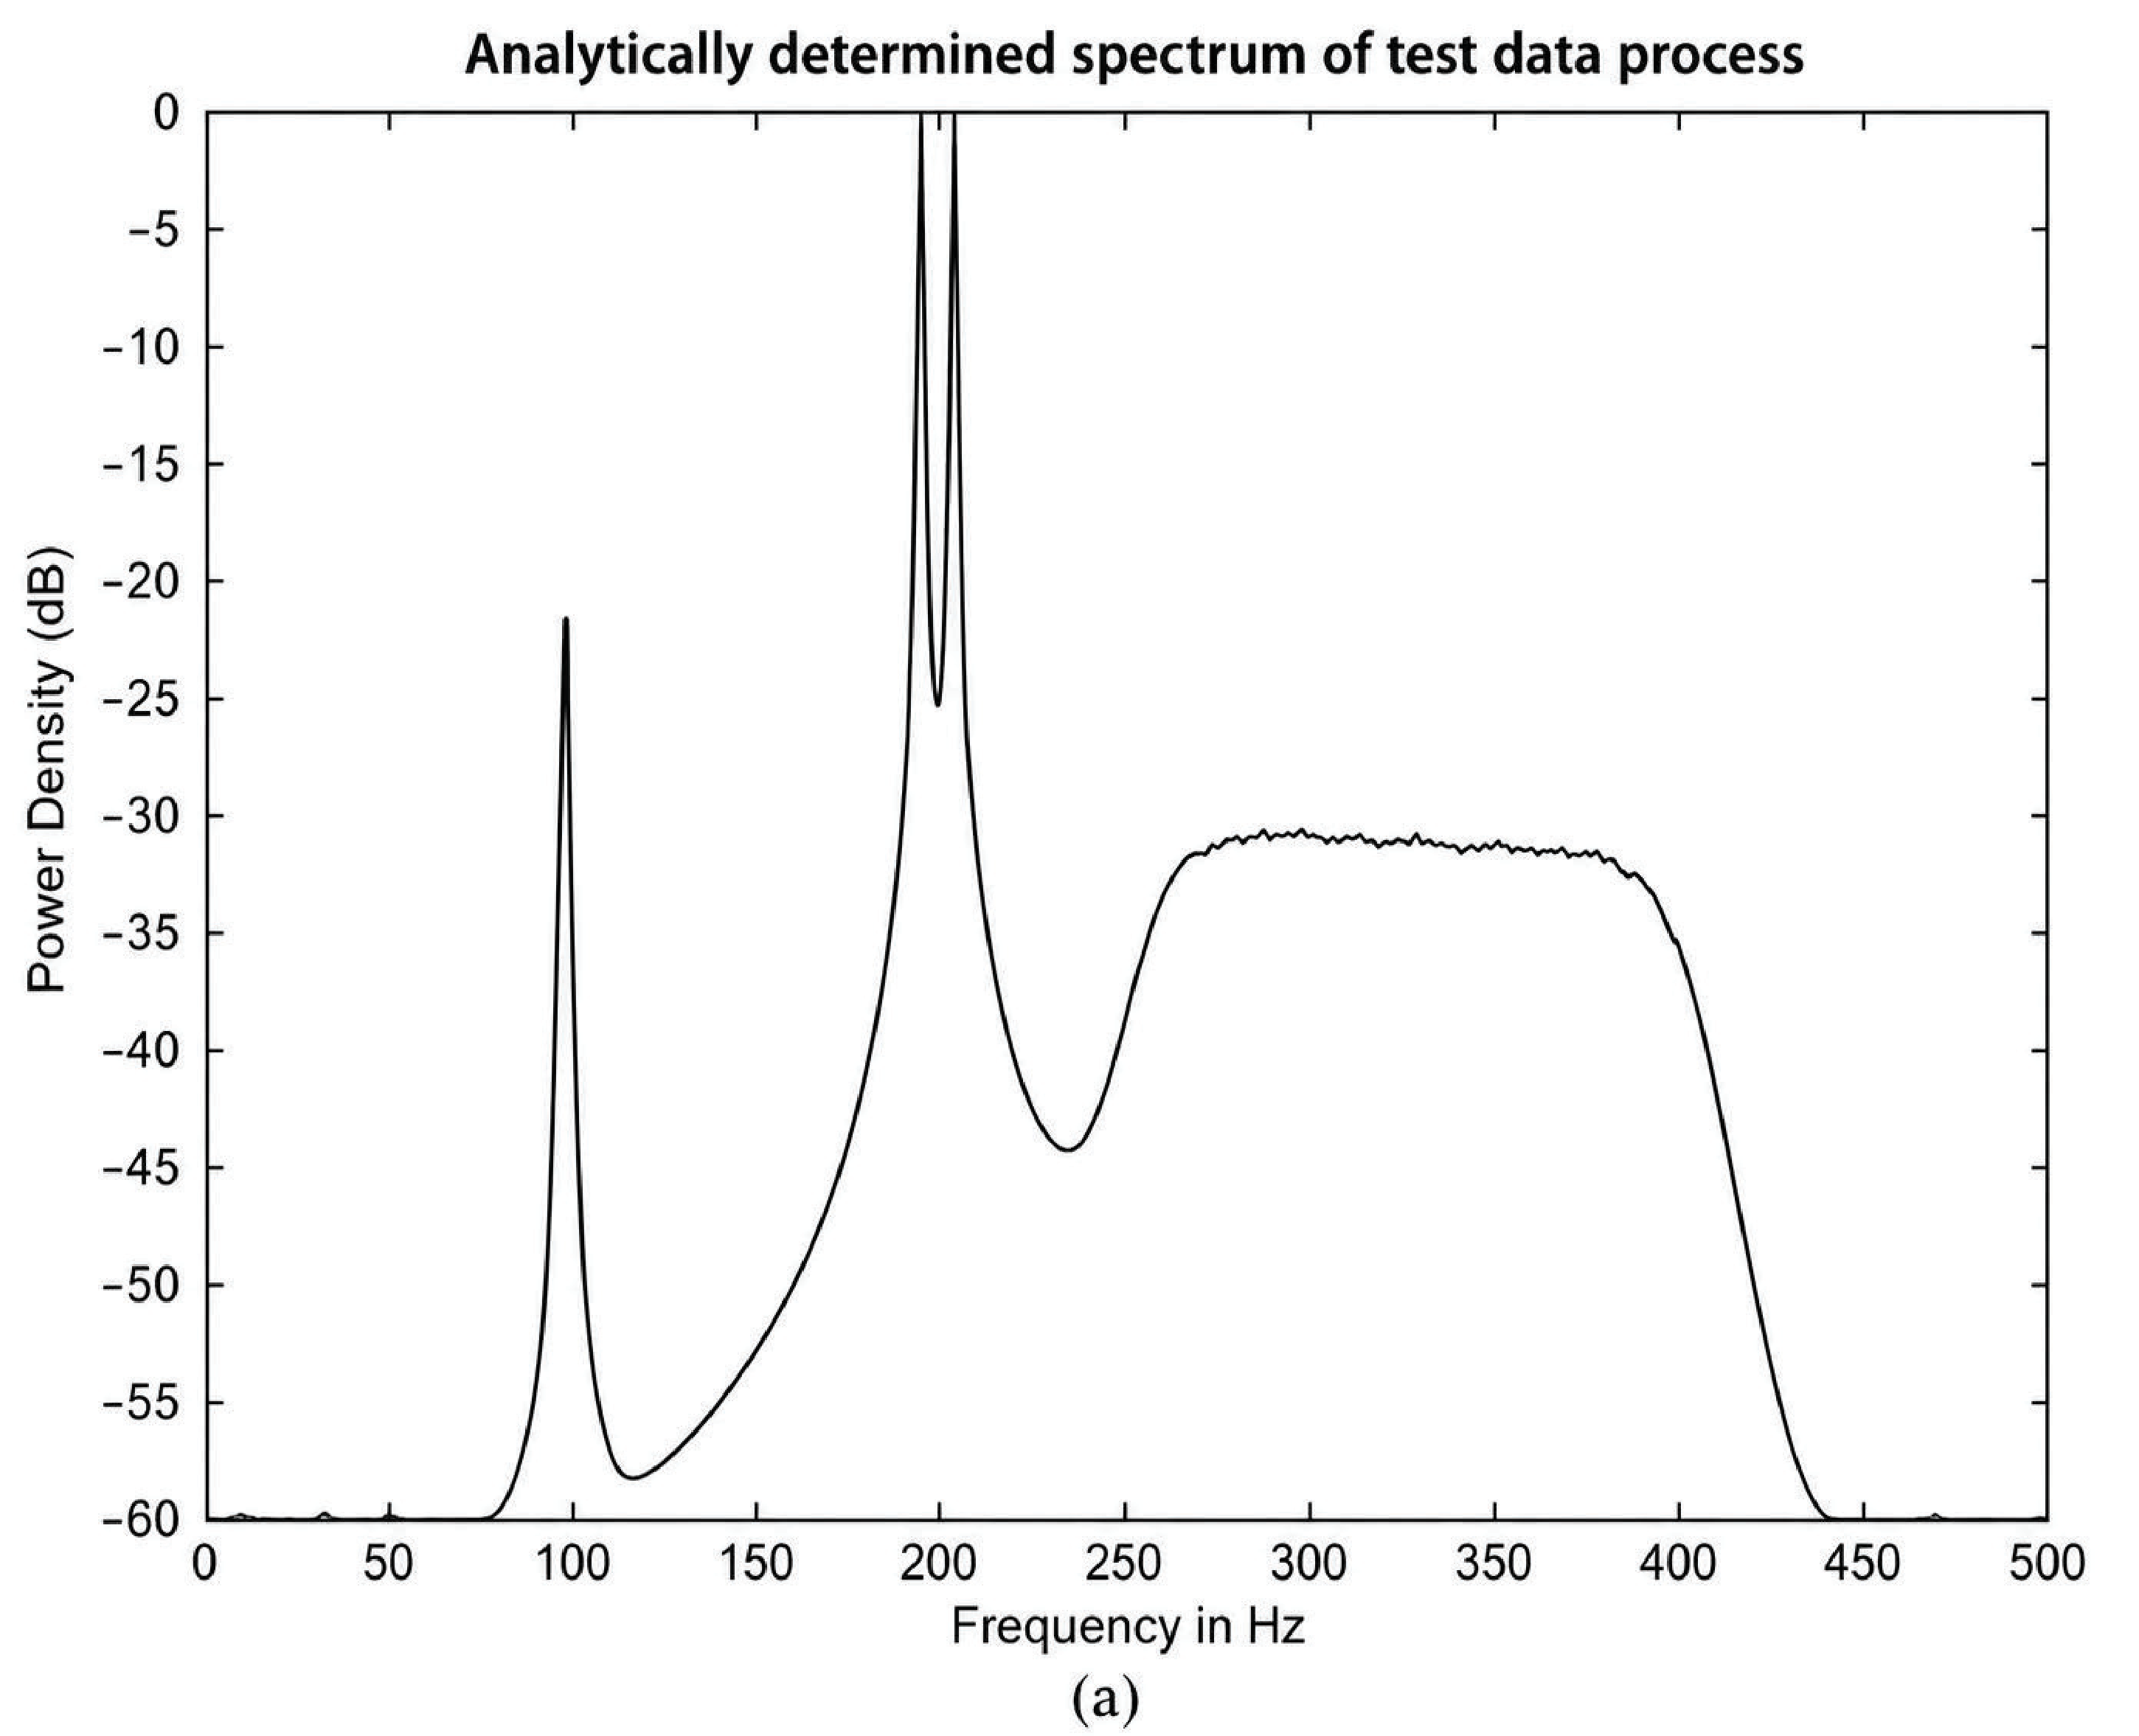
\includegraphics[width=7cm,height=6cm]{Images/reconstructed_top_1_a-eps-converted-to.pdf}
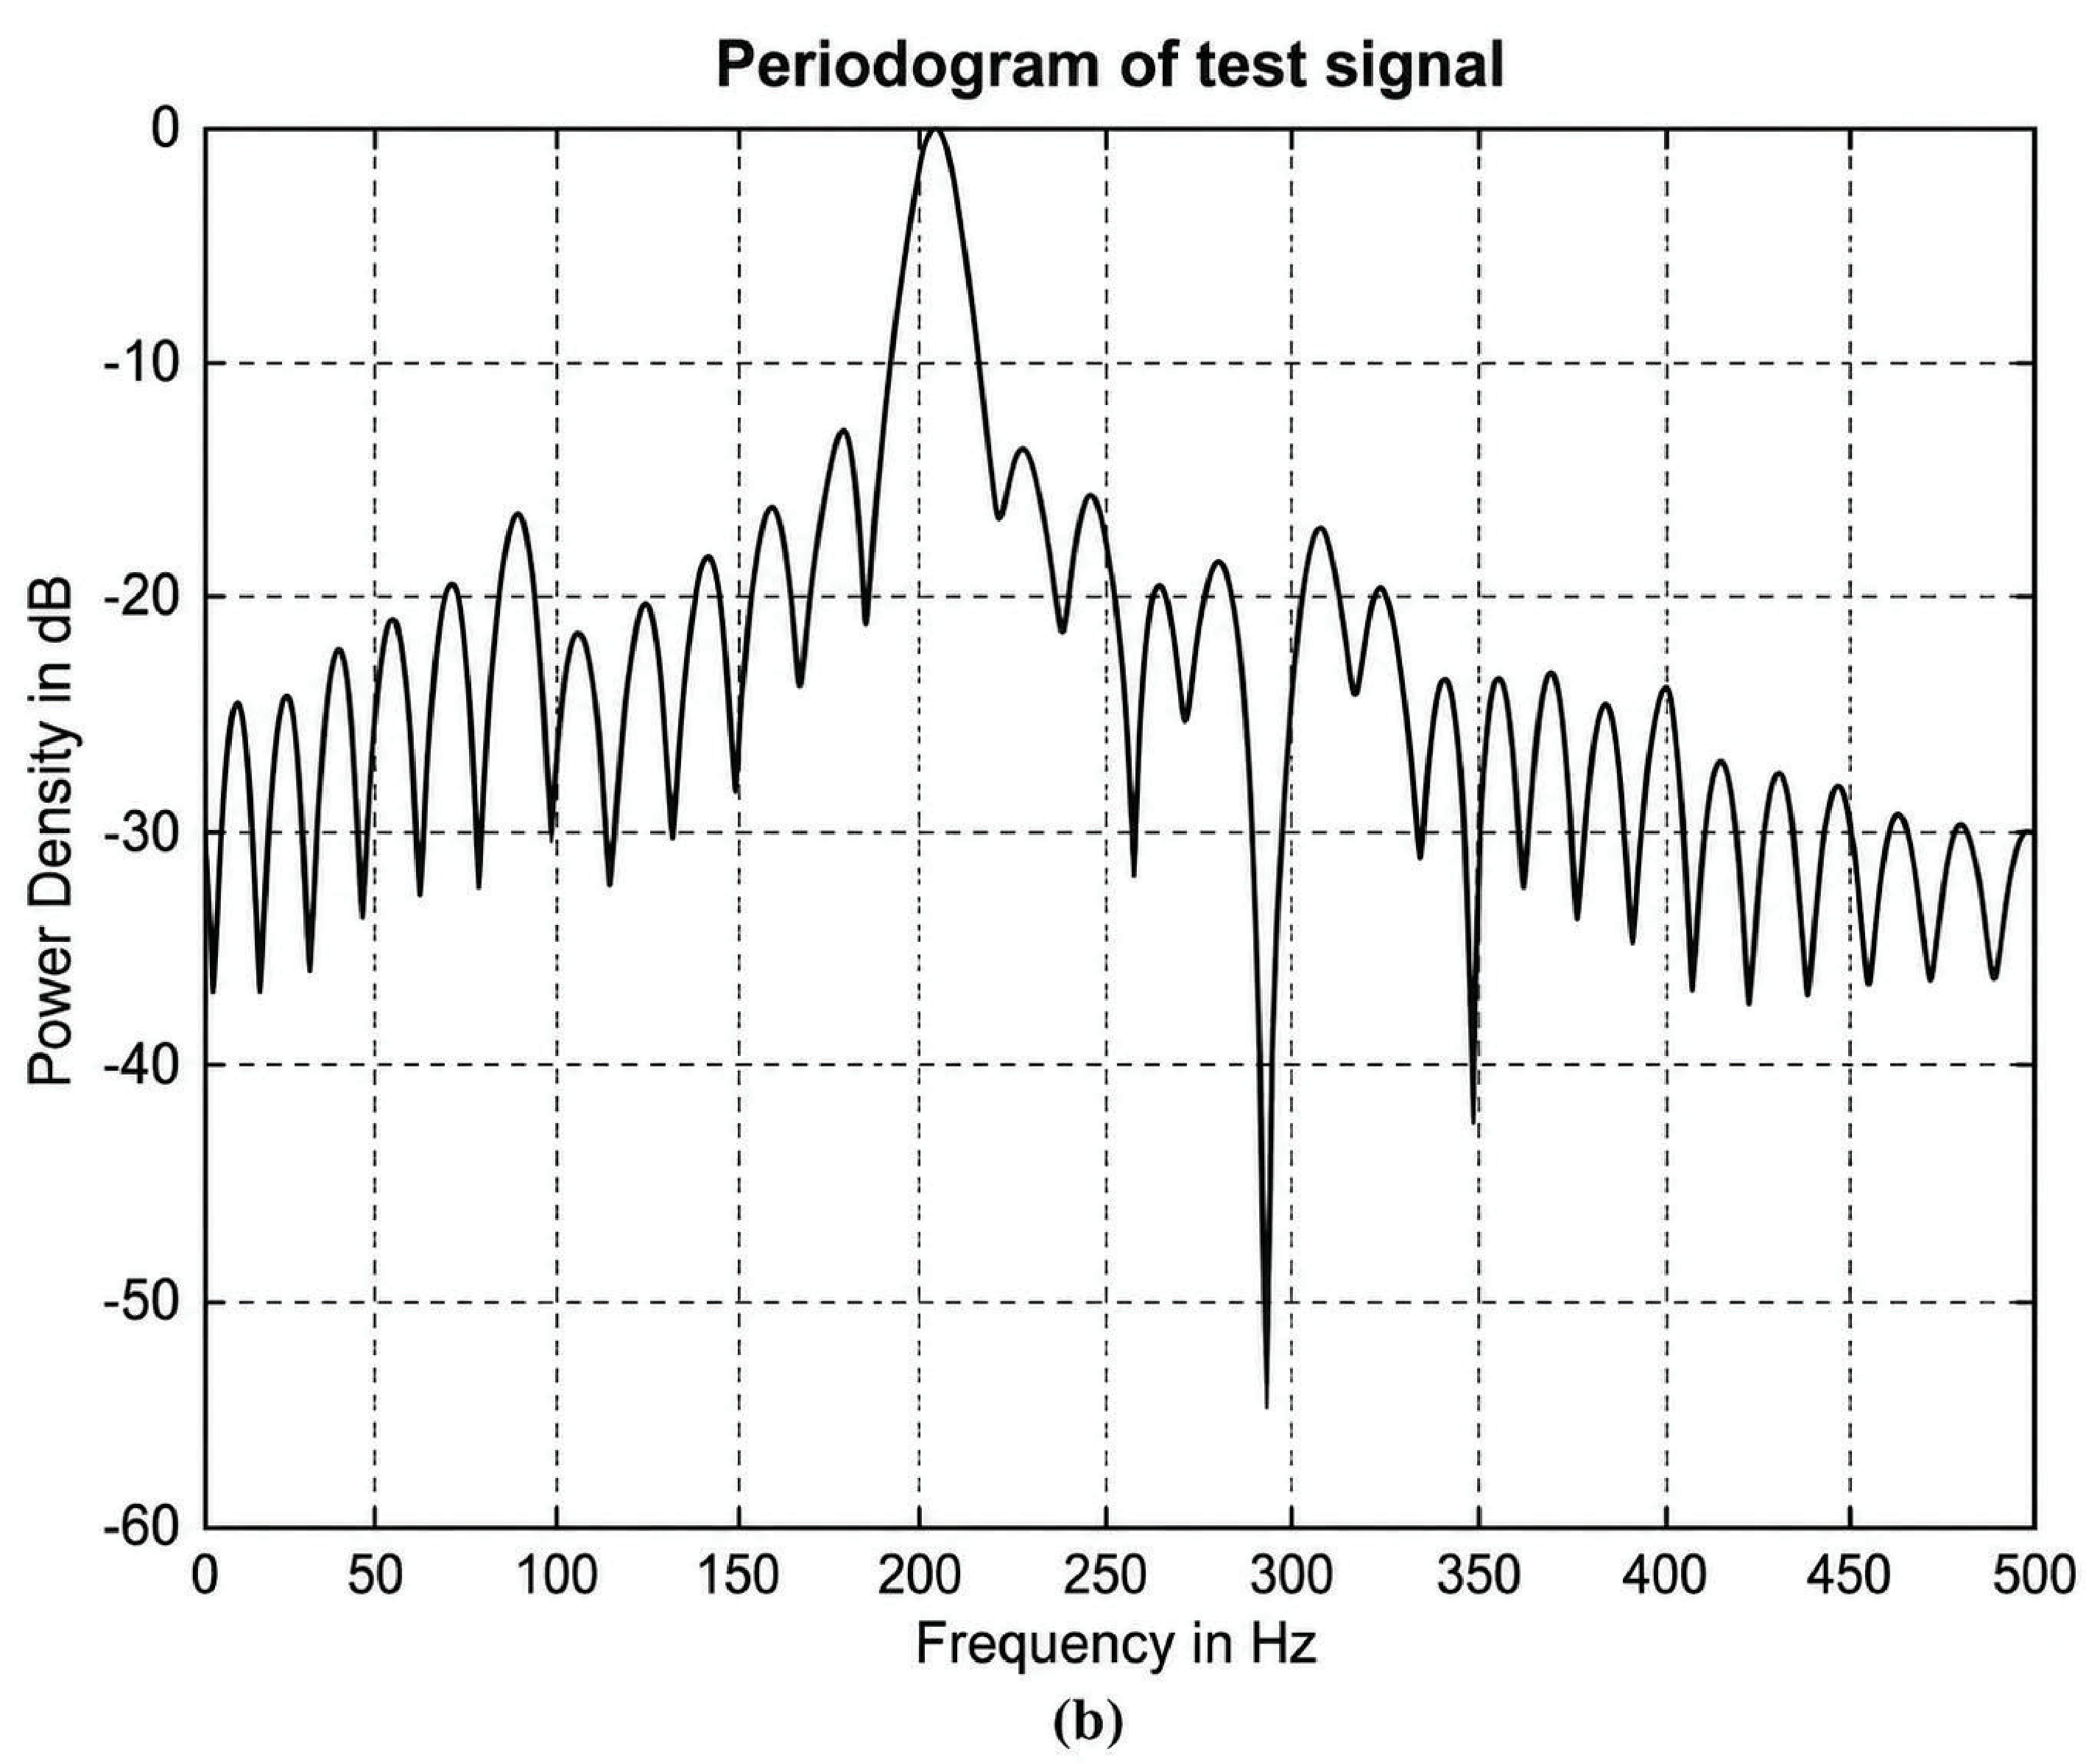
\includegraphics[width=7cm,height=6cm]{Images/reconstructed_top_2_b-eps-converted-to.pdf}
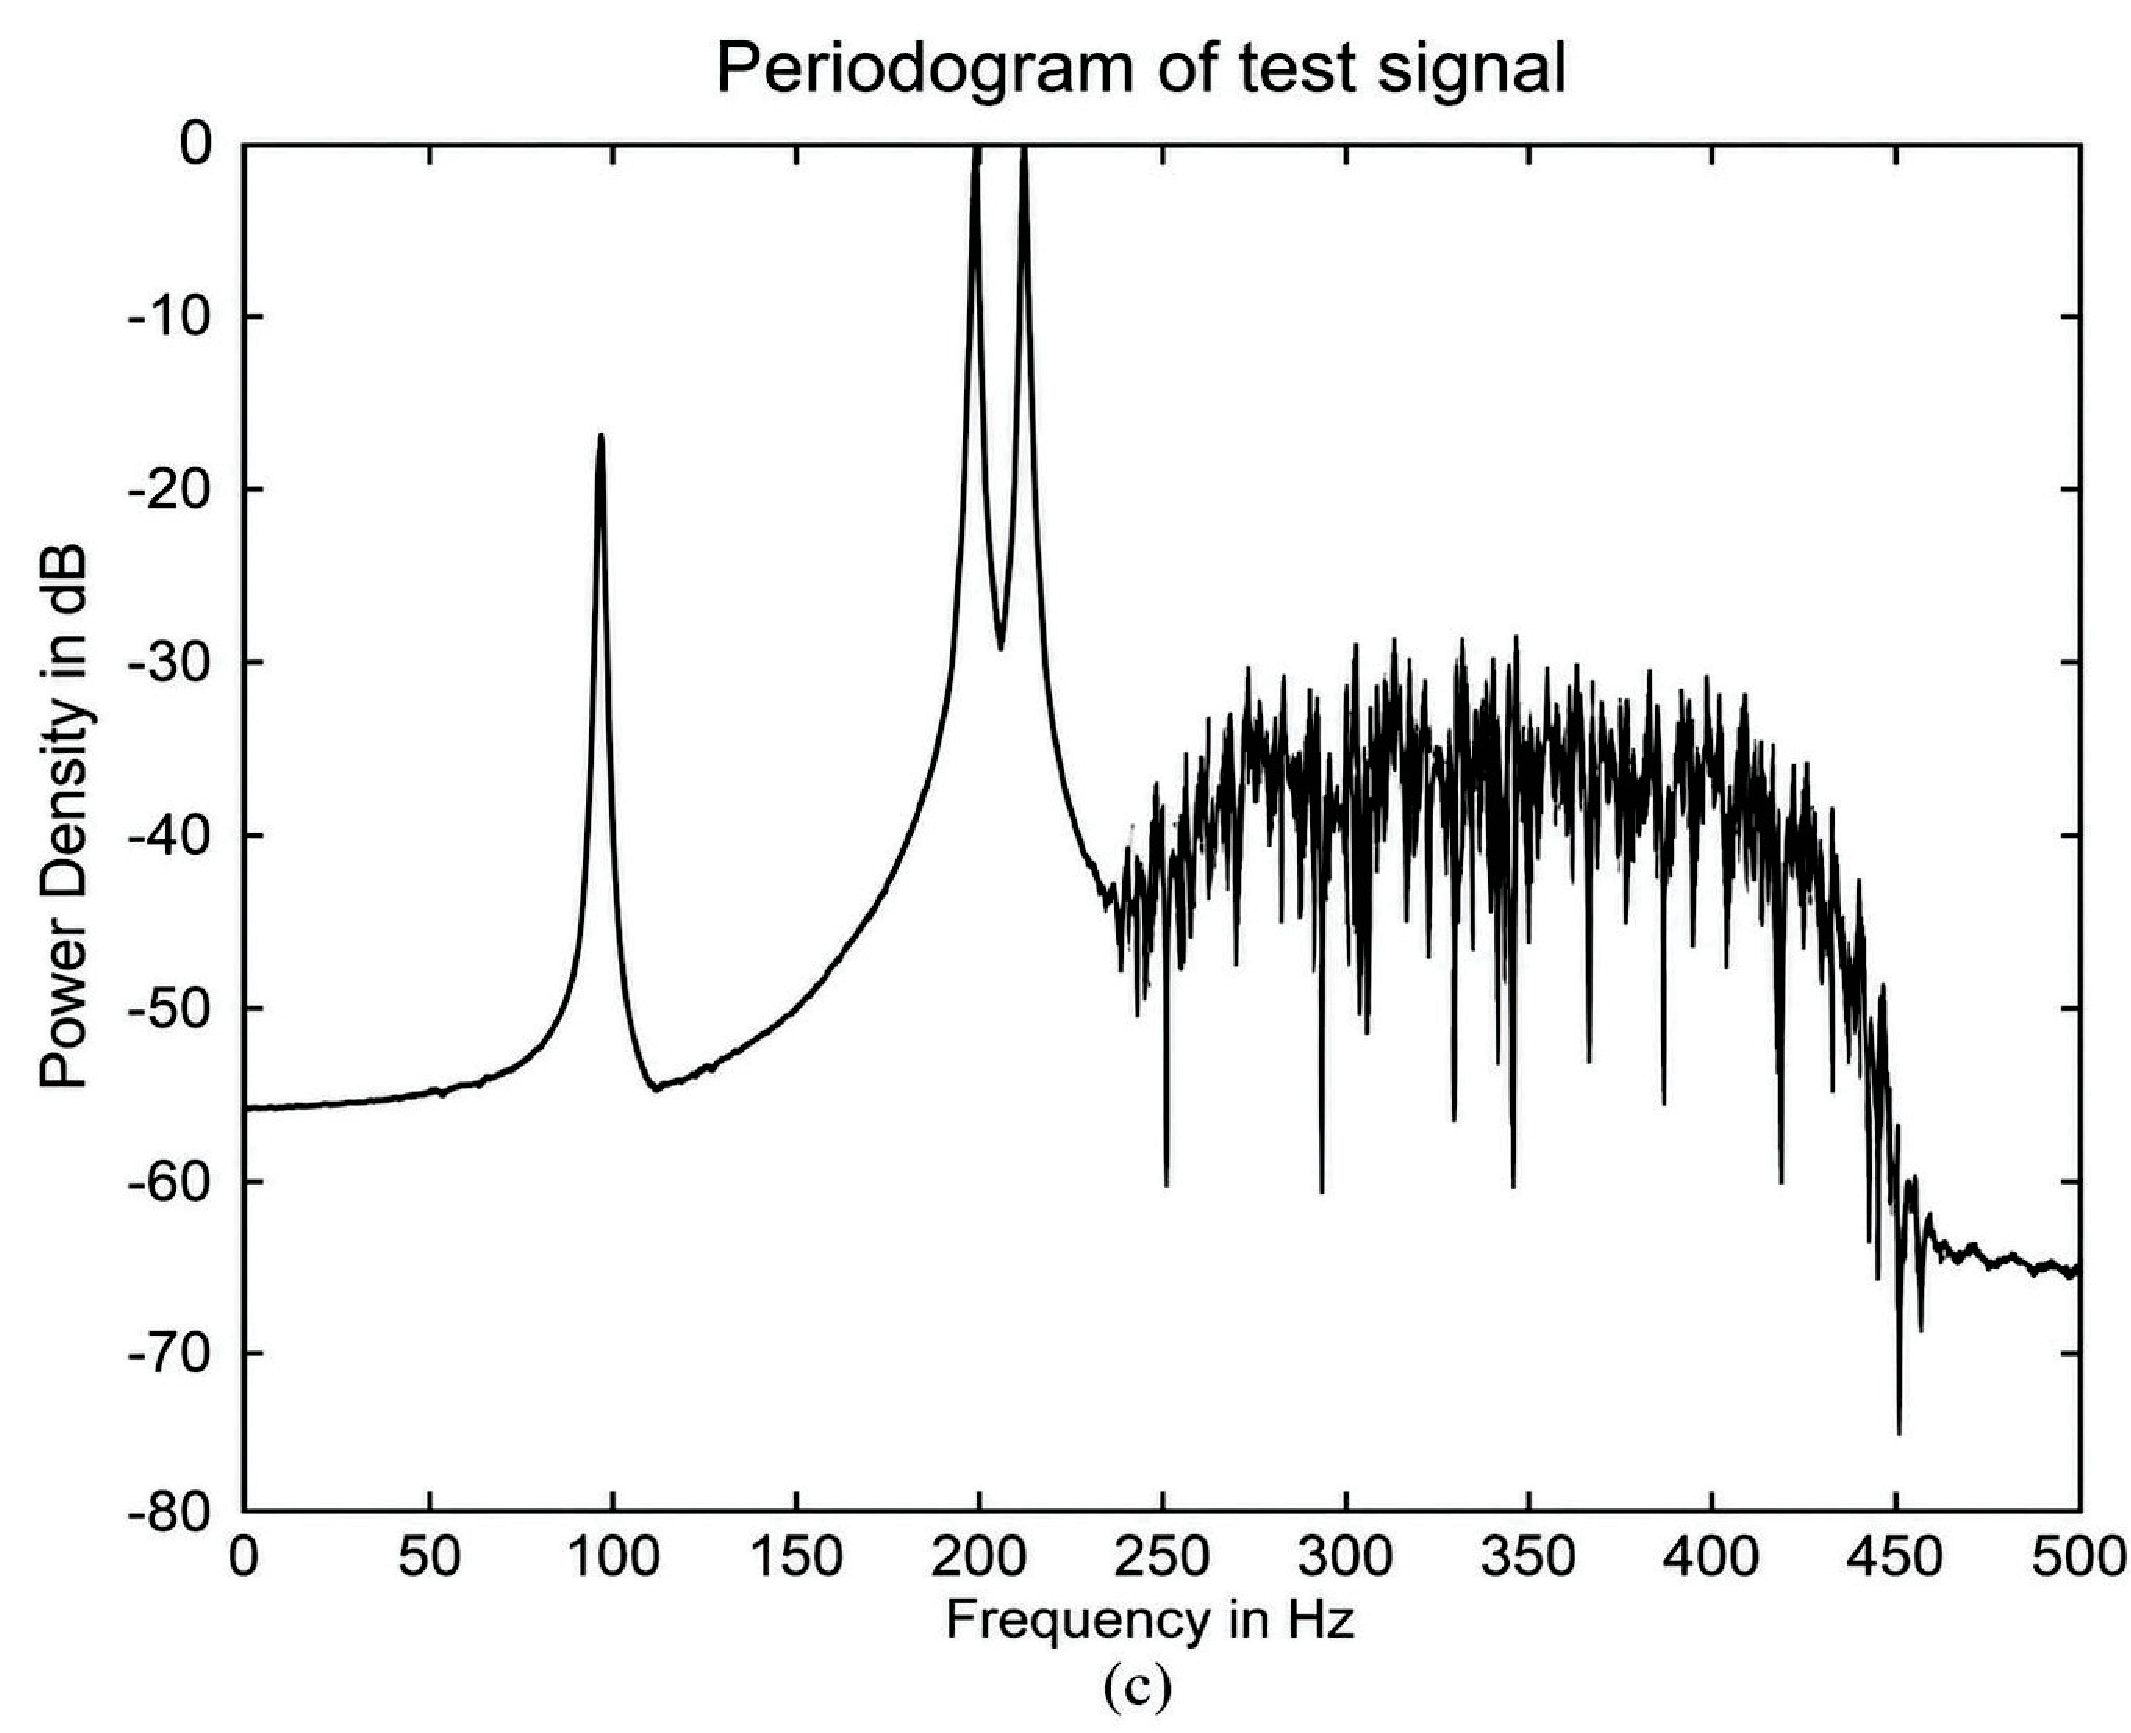
\includegraphics[width=7cm,height=6cm]{Images/reconstructed_bottom_1_c-eps-converted-to.pdf}
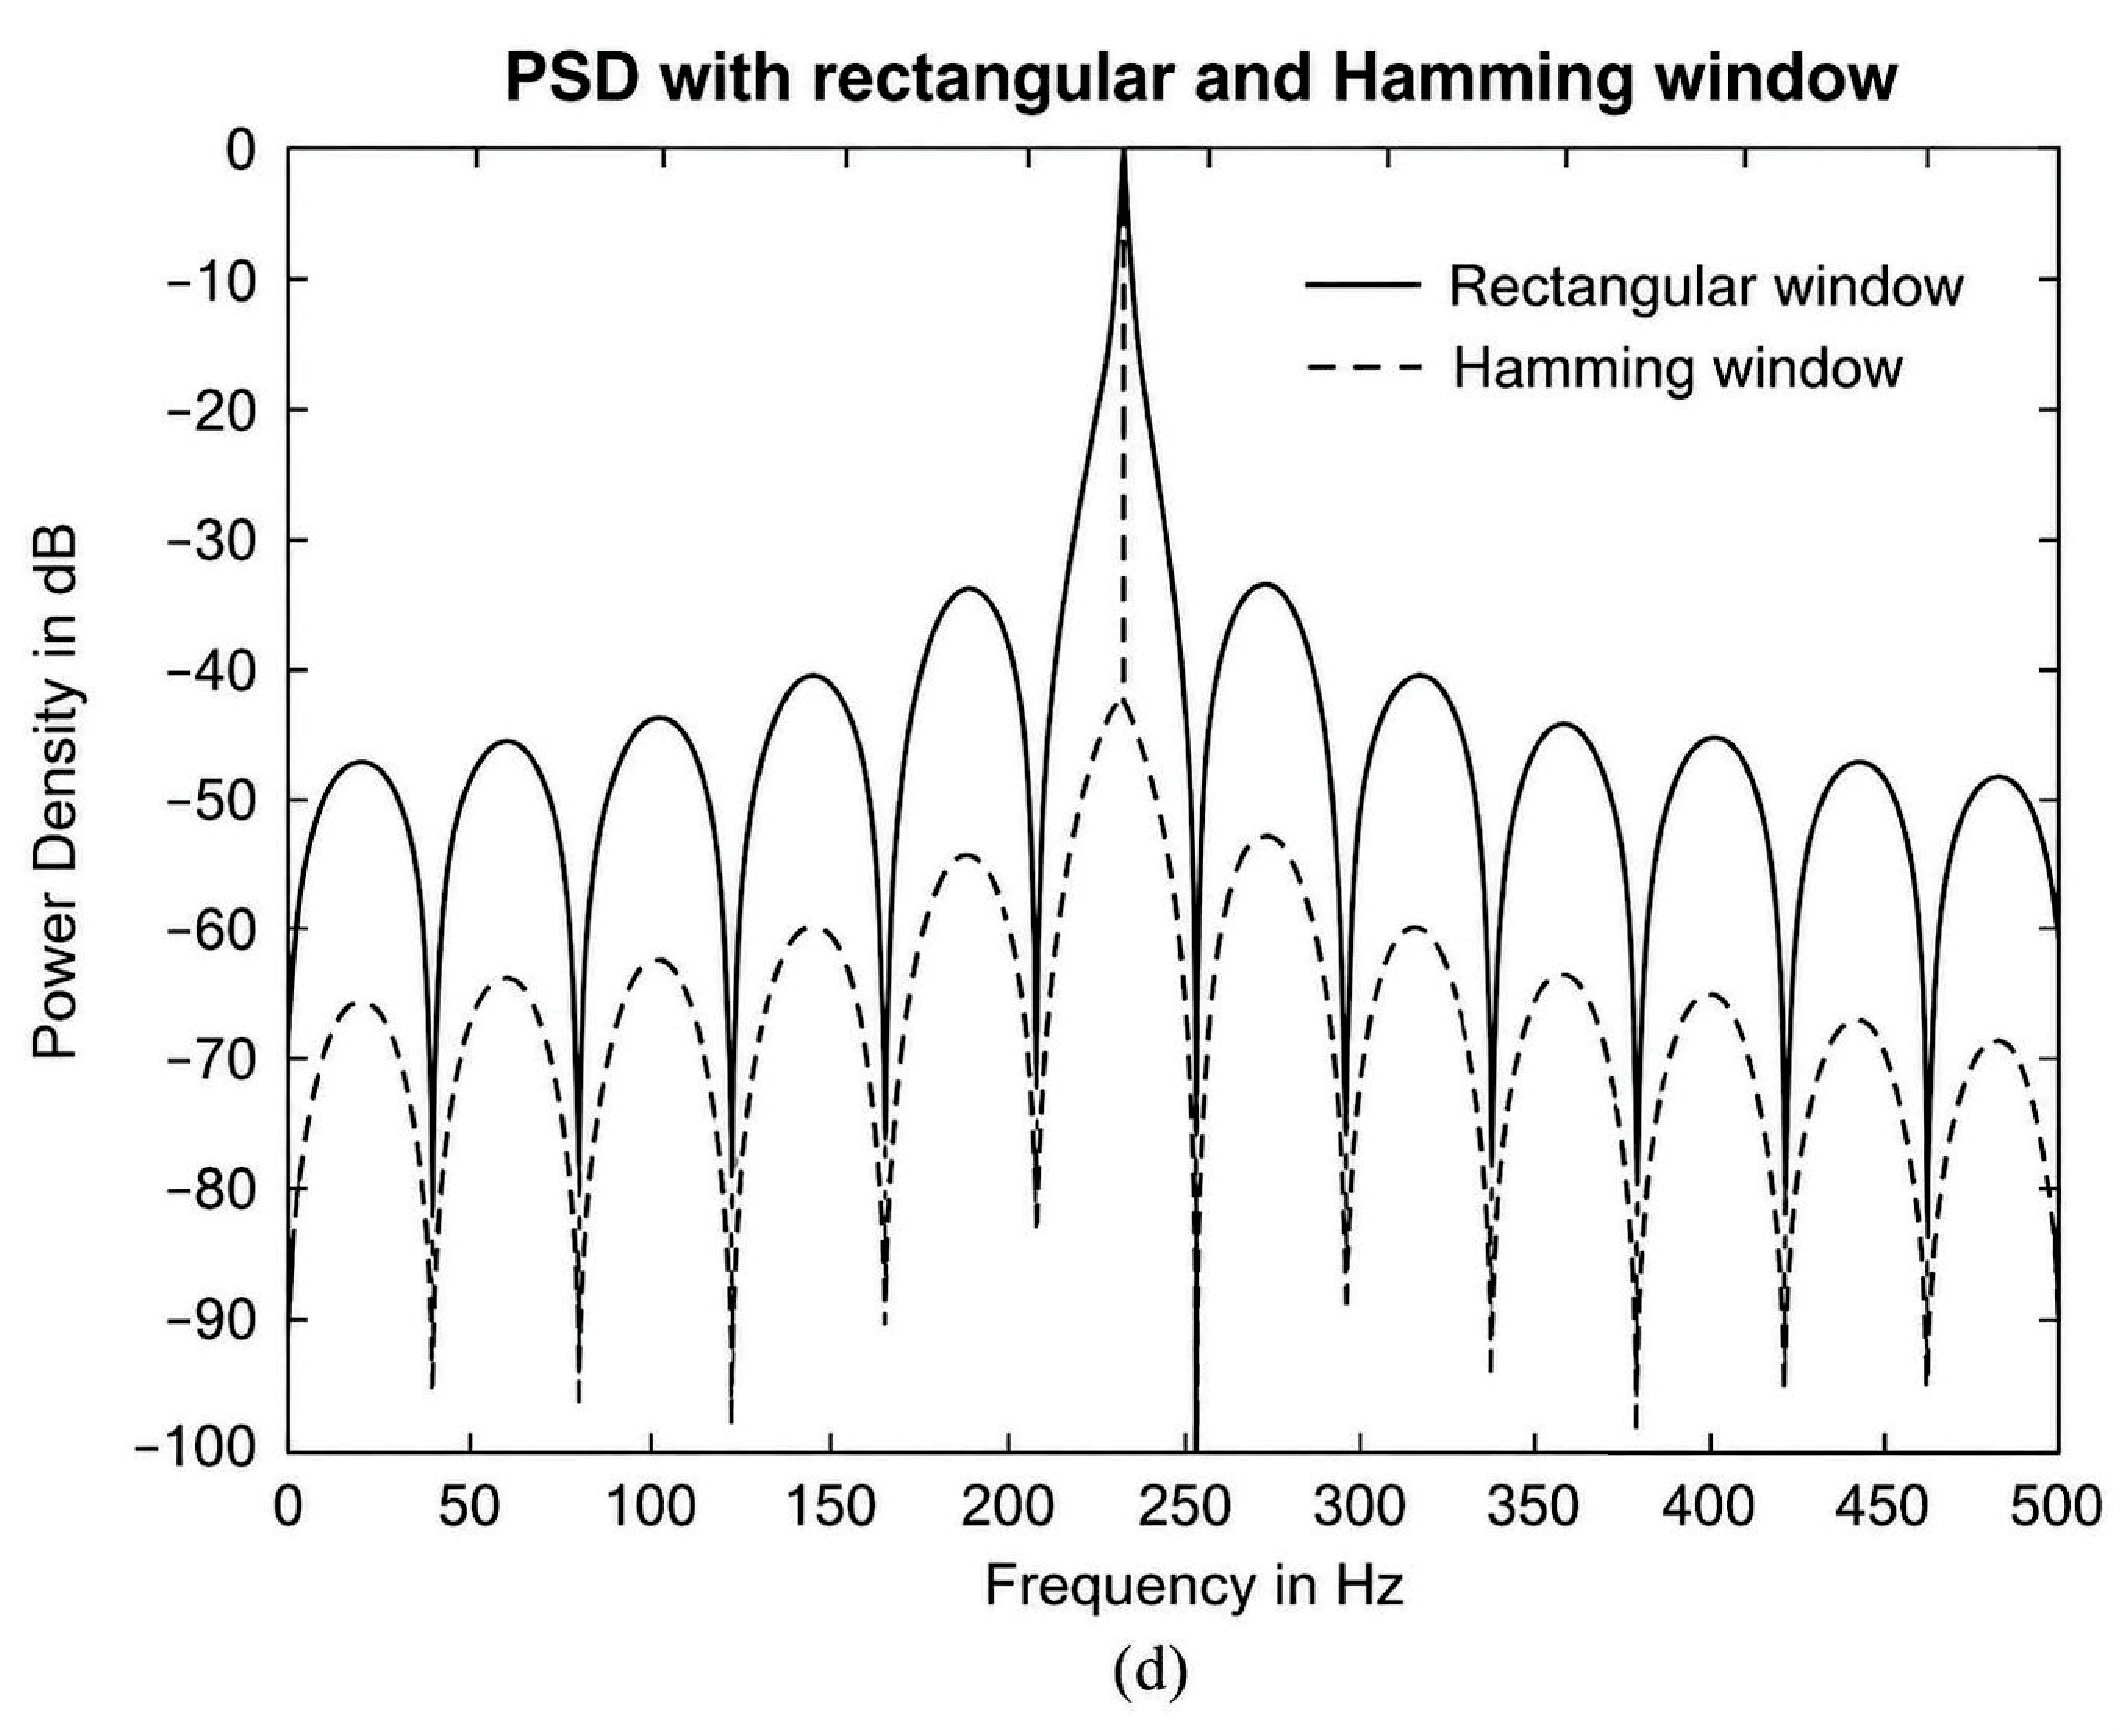
\includegraphics[width=7cm,height=6cm]{Images/reconstructed_bottom_2_d-eps-converted-to.pdf}
%\vspace{-0.2cm}
\caption{\footnotesize{Comparison of classical nonparametric spectral estimates for a signal with two closely-spaced peaks ($0.4\pi$, $0.42\pi$): (a) Theoretical PSD, (b) Periodogram ($n=64$), (c) Periodogram ($n=2048$), (d) Windowed estimates ($n=1000$). The periodogram fails to resolve the peaks for small $n=64$.}}
\label{fig1}
\end{center}
\end{figure}



In contrast, the high-resolution MUSIC algorithm, shown in Figure \ref{fig2}, successfully resolves the spectral components even with only $n=64$ data points. Rather than relying solely on Fourier transforms, MUSIC exploits the subspace structure of the signal, effectively bypassing the resolution limits of classical methods. This comparison shows that while traditional approaches work well for signals with smooth, continuous spectra, high-resolution techniques truly shine when dealing with narrow-band periodic components, especially when data is limited.



\begin{figure}[ht]
\begin{center}
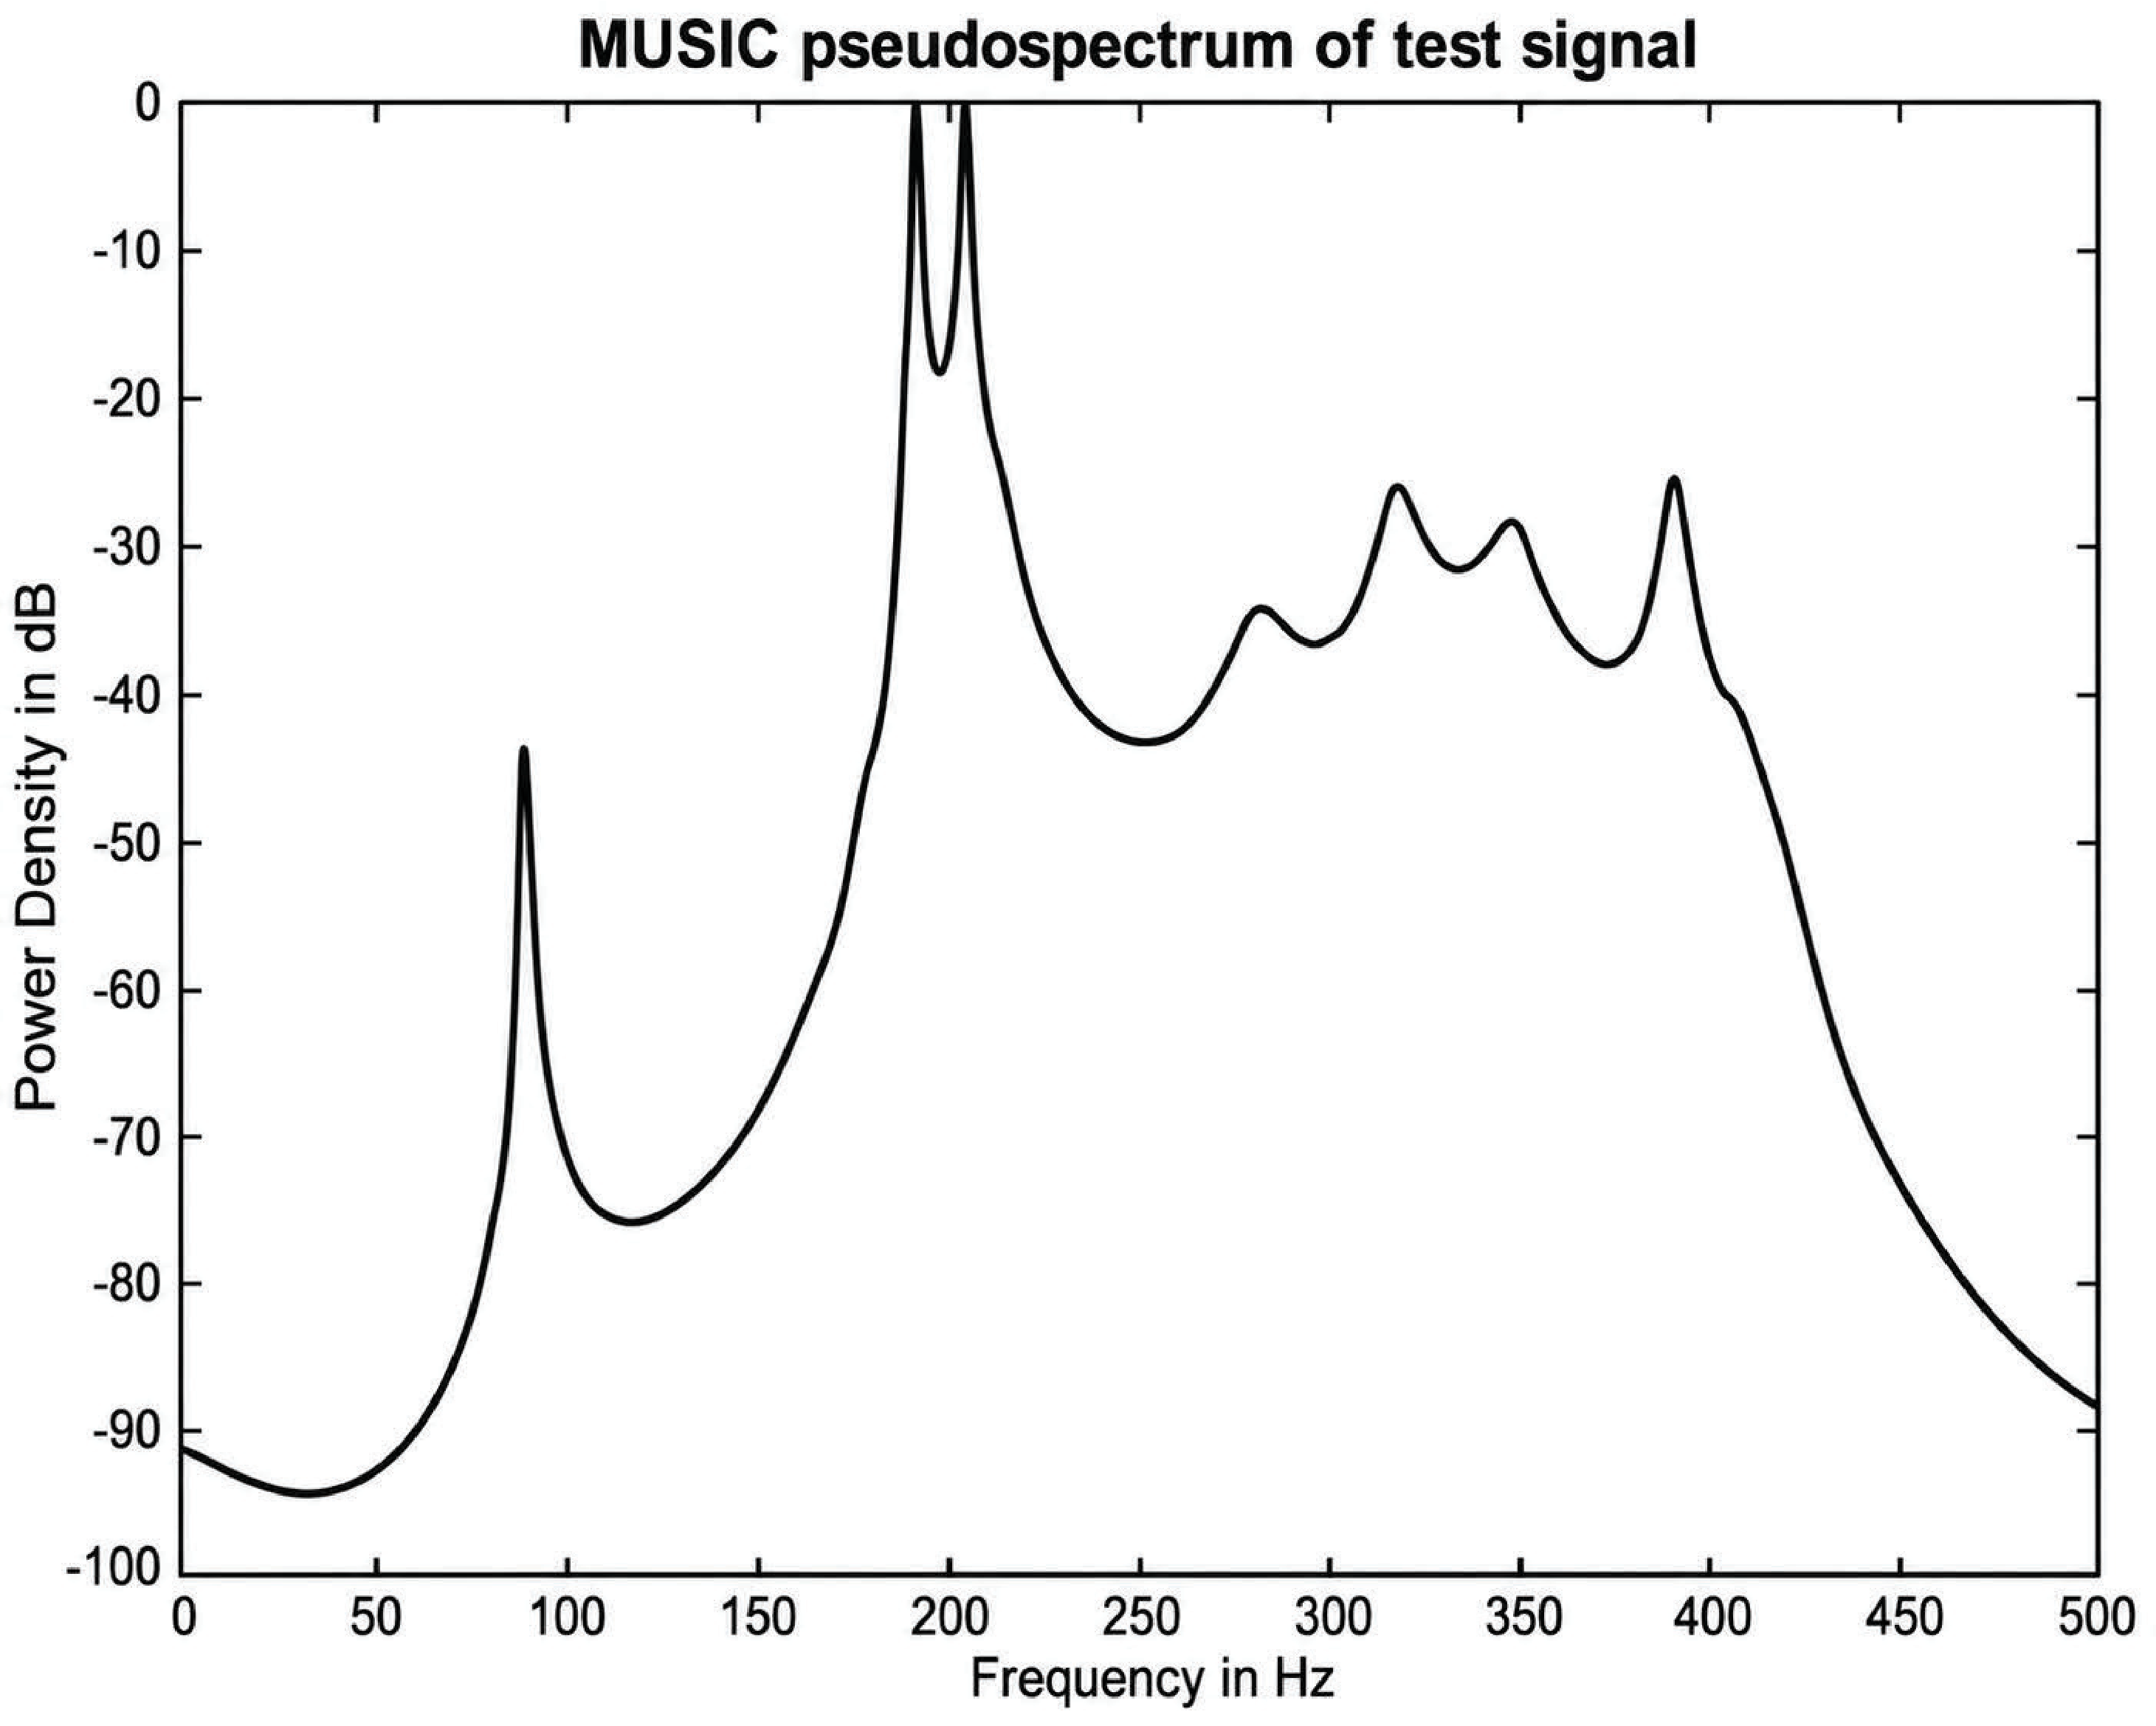
\includegraphics[width=8cm,height=7cm]{Images/reconstructed_Fig2-eps-converted-to.pdf}
%\vspace{-0.2cm}
\caption{\footnotesize{MUSIC spectral estimate for the synthetic signal with $n=64$. The two peaks at $0.4\pi$ and $0.42\pi$ are clearly resolved, demonstrating the superiority of high-resolution methods over classical approaches (Figure 1).}}
\label{fig2}
\end{center}
\end{figure}



Overall, two things are worth highlighting here:
\begin{itemize}
\item \textbf{Resolution Power:} Unlike nonparametric methods, where variance doesn't decrease with more data (leading to inconsistent estimates), high-resolution approaches use the model structure to achieve much sharper resolution.
\item \textbf{Trade-offs:} MLARMA, Capon, and MUSIC offer excellent resolution, but at the cost of higher computational demand. The right choice ultimately depends on whether frequency resolution or computational speed is more important for the task at hand.
\end{itemize}



\section{Extension to the Multivariate Case}
The spectral estimation of a $T$-dimensional stationary process $\{\mathbf{X}_t\}$ involves estimating the spectral density matrix $\mathbf{h}(\omega) = [h_{j,k}(\omega)]$, where each element is defined by the Fourier transform of the cross-covariance function $R_{j,k}(\tau)$. A standard estimator for this matrix is the periodogram matrix $\mathbf{I}_n(\omega)$, which is asymptotically unbiased but remains inconsistent. To achieve consistency, smoothing via a kernel or an eigenvalue-based approach is required.



\subsection{Eigenvalue-Based Multivariate Estimation}



Building upon the work of \cite{SubbaRaoGabr:1989}, a robust framework for multivariate spectral estimation is proposed by \cite{NematollahiSubbaRao:2005} through the spectral decomposition of the block-Toeplitz autocovariance matrix $\mathbf{\Gamma}_n$. They demonstrated that the spectral density matrix $\mathbf{h}_n(\omega)$ can be represented as a function of the "eigenvalue-matrices" $\{\mathbf{\Lambda}_n(\omega_j)\}$ of $\mathbf{\Gamma}_n$. Specifically, they established an approximation relating $\mathbf{h}_n(\omega)$ to the Fejér kernel $F_n(\theta)$:



\begin{equation}
\mathbf{h}_n(\omega_l) = \frac{1}{4\pi} \sum_{j=0}^{n-1} \mathbf{A}_n(\omega_j, \omega_l),
\end{equation}
where $\mathbf{A}_n$ represents the interaction between the eigenvalue-matrices and the Fejér kernel, see \cite{NematollahiSubbaRao:2005} for more details. This expression reveals that $\mathbf{h}_n(\omega)$ is a smooth function of $\mathbf{\Lambda}_n(\omega_j)$, effectively suggesting thatnon-linear transformations of these eigenvalues can be used to construct more precise estimators. By defining a strictly monotonic function $G(\cdot)$ and its inverse $g(\cdot)$, one can generalize the univariate Pisarenko estimator to the multivariate case:
\begin{equation}
\mathbf{h}_{n,P}(\omega_l) = g\left( \sum_{j=0}^{n-1} \frac{2}{n} \mathbf{B}_n^*(\omega_j, \omega_l) G(\mathbf{A}_n(\omega_j)) \mathbf{B}_n(\omega_j, \omega_l) \right),\end{equation}
where $\mathbf{B}_n$ denotes the associated block-transform matrix, and the superscript $*$ denotes the conjugate transpose operator, i.e., $U^* = \overline{U^{\mathsf{T}}}$.



\subsection{Multivariate High-Resolution (Capon) Estimation}



\cite{NematollahiSubbaRao:2005} further extended the Capon (Minimum Variance) estimator to the multivariate domain. The generalized multivariate Capon estimator is given by:
\begin{equation}
\mathbf{h}_{\mathrm{Cap}}(\omega) = \frac{1}{\pi} \left( \frac{2}{n} \mathbf{L}_n^*(\omega) \mathbf{\Gamma}_n^{-1} \mathbf{L}_n(\omega) \right)^{-1},
\end{equation}
where $\mathbf{L}_n(\omega)$ is the multivariate direction vector given by $\mathbf{L}_n(\omega) = (\mathbf{I}, \exp\{i\omega\}\mathbf{I}, \ldots, \exp\{i n \omega\}\mathbf{I})^\mathsf{T}$. They proved that this can be equivalently expressed through the inverse of the eigenvalue-matrices:
\begin{equation}
\mathbf{h}_{\mathrm{Cap}}(\omega_l) = \frac{1}{\pi} \left( \sum_{j=0}^{n-1} \widetilde{\mathbf{A}}_n(\omega_j, \omega_l) \right)^{-1}.
\end{equation}



In this expression, $\widetilde{\mathbf{A}}_n(\omega_j, \omega_l)$ serves as the multivariate weighting matrix that incorporates the inverse eigenvalue-matrix $\mathbf{\Lambda}_n^{-1}(\omega_j)$. By inversely weighting the contributions of the eigen-components of the covariance matrix $\mathbf{\Gamma}_n$, this formulation allows the estimator to suppress noise subspaces and sharpen spectral peaks. Effectively, $\widetilde{\mathbf{A}}_n$ acts as an operator that transforms the eigenvalue decomposition into a high-resolution spectral density matrix, directly generalizing the univariate MVS estimator given by (\ref{eq:pisarenko}) with $G(x) = x^{-1}$.



This formulation provides a rigorous statistical basis for multivariate high-resolution analysis, demonstrating that the MV estimator is essentially a non-linear operation on the eigenvalues of the autocovariance matrix.



\section{Applications and Further Perspectives}



Spectral estimation plays a key role across many scientific and engineering fields. While it has long been used in areas like geophysics and classical physics, its most impactful applications today lie in telecommunications and signal processing, especially when it comes to high-resolution target characterization.



Among the high-resolution methods, the MUSIC algorithm stands out and is widely used for Direction-of-Arrival (DoA) estimation and frequency-based signal detection. Some of the main applications include:



\begin{itemize}
\item \textbf{Signal Intelligence and Monitoring}: By examining the Power Spectral Density (PSD), we can tell the difference between background noise and actual signals. Sharp peaks in the spectrum usually indicate active transmitters, which helps in detecting unauthorized or hidden communication sources.
\item \textbf{Target Localization}: In radar and sonar systems, spectral estimation helps determine where a target is located. Whether it's tracking a mobile device in a busy city or detecting underwater objects, these systems rely on frequency shifts and angular information to locate and follow moving targets.
\item \textbf{System Identification}: Beyond just detection, spectral analysis gives us insight into how a system behaves over time. By looking at its frequency response, engineers can spot recurring patterns in vibrations or environmental changes, which is essential for both maintenance planning and fault diagnosis.
\end{itemize}



In all these cases, the ability to separate very close spectral peaks is what makes accurate detection possible.



The relationship between AR-based spectra and Capon-type estimators has been also extended to 2D time series, with significant applications in image processing and Synthetic Aperture Radar (SAR) imagery (see \cite{Larsonetal:2003} and \cite{StoicaMoses:2005}). These 2D extensions allow for complex signal characterization in spatial-temporal domains, proving that the principles of high-resolution spectral estimation are adaptable to higher-dimensional data structures.



Advanced frameworks have further integrated these robust estimation techniques into adaptive beamforming for modern wireless communication systems and high-dimensional spectral analysis (e.g., \cite{LiStoica:2005}, \cite{StoicaMoses:2005}, \cite{Iranietal:2026} and \cite{Haoetal:2026}). These contemporary approaches continue to leverage the fundamental eigenvalue-based frameworks to enhance resolution in non-stationary and large-scale data environments.



\section*{Discussion and Conclusion}



In this paper, we reviewed the principal approaches to spectral density estimation, transitioning from classical nonparametric methods to advanced high-resolution parametric techniques, and highlighted their natural extensions to multivariate time series analysis.



While classical windowed periodograms remain robust and reliable across broad signal classes, their frequency resolution is fundamentally constrained by the Fourier transform window length. High-resolution techniques, such as the Burg, Capon, and MUSIC algorithms, adopt an alternative paradigm by exploiting the underlying parametric model or the subspace structure of the covariance matrix. Whether through covariance matrix inversion (Capon) or prediction-error minimization (Burg), these approaches effectively sharpen spectral peaks, enabling the resolution of closely spaced frequency components that classical methods would otherwise obscure due to leakage. Consequently, they prove particularly advantageous in data-limited regimes.



By bridging intuitive engineering formulations with rigorous statistical frameworks, such as the asymptotic developments established in \cite{NematollahiSubbaRao:2005}, this study underscores the versatility and robustness of eigenvalue-based spectral estimation methodologies.



Nevertheless, spectral estimation remains an active and evolving field of research. While our primary focus centered on evaluating existing frameworks, several open challenges persist. Future work will investigate the development of computationally efficient, time-recursive implementations of the Capon estimator, alongside data-driven optimization strategies for selecting optimal window functions and smoothing bandwidths. Addressing these challenges will further enhance the practicality and scalability of high-resolution spectral analysis in contemporary real-world signal processing applications.



\begin{thebibliography}{9}



\bibitem[Akaike (1973)]{Akaike:1973}
Akaike, H. (1973). Information theory and an extension of maximum likelihood principle. \textit{2nd International Symposium on Information Theory}, B. N. Petrov and F. Csaki, eds. Akademiai Kiado, Budapest, pp. 267--281.



\bibitem[Brockwell and Davis (1991)]{BrockwellDavis:1991}
Brockwell, P.J. and Davis, R.A. (1991). \textit{Time Series: Theory and Methods}, Springer, New York.



\bibitem[Capon (1969)]{Capon:1969}
Capon, J. (1969). High resolution frequency-wave number spectrum analysis. \textit{Proc. IEEE,} \textbf{57}, 1408--1418.



\bibitem[Carbone (2022)]{Carbone:2022}
Carbone, C. (2022). \textit{Power Spectral Density Estimation by Example: Fundamentals of PSD Estimation Using R}, Independently published, Amazon.



\bibitem[Dumitrescu et al. (2001)]{Dumitrescuetal:2001}
Dumitrescu, B., Tabus, I. and Stoica, P. (2001). On the parametrization of positive real sequences and MA parameter estimation. \textit{IEEE Trans. Signal Process,} \textbf{49}, 2630--2639.



\bibitem[Hao et al. (2026)]{Haoetal:2026}
Hao, F., Yu, B., Cong, Z., Zhang, Y., Pan, S., Yao, Z. and Chen, Y. (2026). Robust broadband adaptive beamforming for planar arrays with tunable nulls in high-dynamic scenario. \textit{Scientific Reports}, \textbf{16}, 8131.



\bibitem[Irani et al. (2026)]{Iranietal:2026}
Irani, K.H, Vorobyov, S.A. and Huang, Y. (2026). Learning-Enhanced Distributionally Robust Adaptive Beamforming, \textit{IEEE International Conference on Acoustics, Speech and Signal Processing (ICASSP)}, Barcelona, Spain, 20726-20730.



\bibitem[Kay (1988)]{Kay:1988}
Kay, S.M. (1988). \textit{Modern Spectral Estimation: Theory and Application}, Prentice-Hall, Englewood Cliffs, NJ.



\bibitem[Larson et al. (2003)]{Larsonetal:2003}
Larson, E.G., Li, J. and Stoica, P. (2003). High-resolution nonparametric spectral analysis: theory and applications. In \textit{High-Resolution Signal Processing}, Y. Hua, Q. Cheng, and A. B. Gershman, eds. Marcel Dekker, New York.



\bibitem[Li and Stoica (2005)]{LiStoica:2005}
Li, J., and Stoica, P. (2005). \textit{Robust Adaptive Beamforming}, John Wiley and Sons.



\bibitem[Marple (1987)]{Marple:1987}
Marple, S.L. (1987). \textit{Digital Spectral Analysis with Applications}, Englewood Cliffs, NJ: Prentice-Hall.



\bibitem[Mewes and Dermühl (2001)]{MewesDermühl:2001}
Mewes, H. and Dermühl, M. (2001). Improvement on high resolution spectral estimation techniques in sensor array signal processing, Unpublished manuscript.





\bibitem[Nematollahi and Subba Rao (2005)]{NematollahiSubbaRao:2005}
Nematollahi, A.R. and Subba Rao, T. (2005). On the spectral density estimation of periodically correlated (cyclostationary) time series. \textit{Sankhy\={a} Ser. A,} \textbf{67}, 568--589.



\bibitem[Percival and Walden (1993)]{PercivalWalden:1993}
Percival, D.B. and Walden, A.T. (1993). \textit{Spectral Analysis for Physical Applications: Multilayer and Conventional Univariate Techniques}, Cambridge University Press, Cambridge, UK.



\bibitem[Pisarenko (1972)]{Pisarenko:1972}
Pisarenko, V.F. (1972). On the estimation of spectra by means of nonlinear functions of the covariance matrix. \textit{Geophys. J. R. Astr. Soc.}, \textbf{28}, 511--531.



\bibitem[Priestley (1962)]{Priestley:1962}
Priestley, M.B. (1962). Basic considerations in the estimation of spectra. \textit{Technometrics} \textbf{4}, 551--564.



\bibitem[Shumway and Stoffer (2025)]{ShumwayStoffer:2025}
Shumway, R. H. and Stoffer, D. S. (2025). \textit{Time Series Analysis and Its Applications: With R Examples}, Fifth Edition, Springer, Cham.



\bibitem[Stoica et al. (2000)]{Stoicaetal:2000}
Stoica, P., McKelvey, T. and Mari, J. (2000). MA estimation in polynomial time. \textit{IEEE Trans. Signal Process,} \textbf{48}, 1999--2012.



\bibitem[Stoica and Moses (1997)]{StoicaMoses:1997}
Stoica, P. and Moses, R.L. (1997). \textit{Introduction to Spectral Analysis}, Prentice-Hall, NJ.



\bibitem[Stoica and Moses (2005)]{StoicaMoses:2005}
Stoica, P. and Moses, R.L. (2005). \textit{Spectral Analysis of Signals}, Prentice-Hall, NJ.



\bibitem[Subba Rao and Gabr (1989)]{SubbaRaoGabr:1989}
Subba Rao, T. and Gabr, M.M. (1989). The estimation of spectrum, inverse spectrum and inverse autocovariances of a stationary time series. \textit{J. Time Ser. Anal.}, \textbf{10}, 183--202.



\end{thebibliography}
 \end{document}





